\chapter{Results}

\section{Data Collected}

    Data on the output of the engine and its temperature was recorded and plotted, as seen in Figure \ref{fig:data3}. Temperature data was taken every 200ms, while voltage was taken every 5ms.
    
    \begin{figure}[ht]
        \centering
        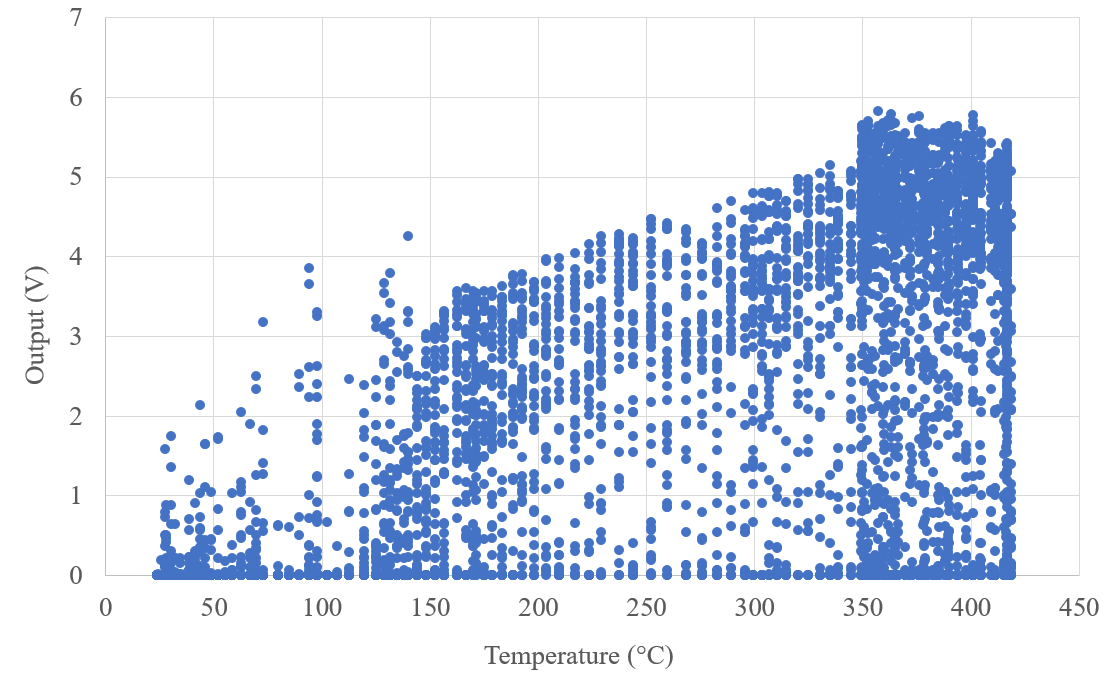
\includegraphics[width=\textwidth]{diagrams/data3}
        \caption[Data]{Output voltage versus Stirling engine temperature.}
        \label{fig:data3}
    \end{figure}
    
    Additionally it is possible to plot the output by time, as seen in Figure \ref{fig:timedata}. While this does not give information regarding the relationship between temperature and output, it is easier to see how the output changes over time:
    
    \begin{figure}[ht]
        \centering
        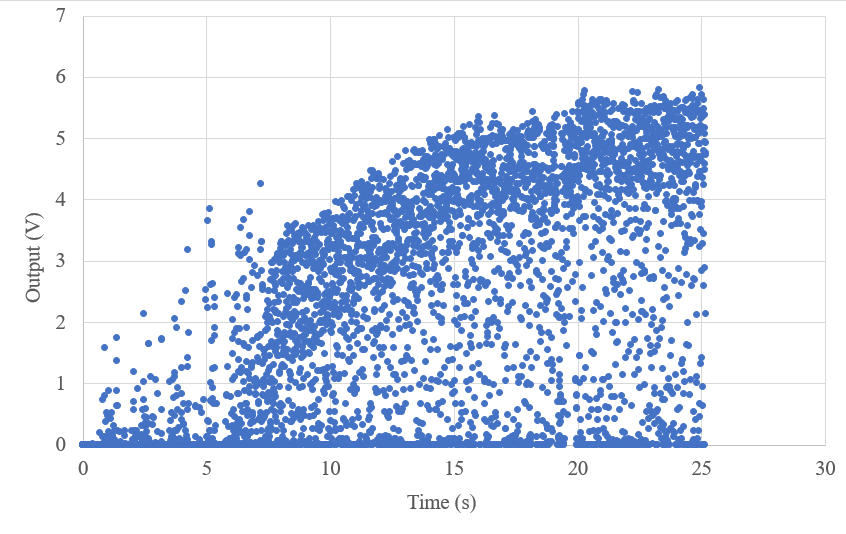
\includegraphics[width=\textwidth]{diagrams/timedata}
        \caption[Time-dependent data]{Output voltage versus time elapsed during data collection.}
        \label{fig:timedata}
    \end{figure}

\section{Analysis}
    
    This data appears noisy due to the A.C. output by the generator. A rectifier was placed with the output of the motor in order to turn negative voltages in to positive, thus the data here resembles a function:
    
    \begin{equation}
        V(t) = \lvert V_{max}(t) \sin(\omega t) \rvert
        \label{eqn:sin}
    \end{equation}
    Where $V_{max}(t)$ is an increasing amplitude by time and $\omega$ is the angular frequency $2\pi f$, dependent on the angular velocity of the generator (i.e. how fast it is spinning). The rectifier thus changes the sinusoidal function from Figure \ref{fig:emfsine} to resemble the following:
    
    \begin{figure}[H]
        \centering
        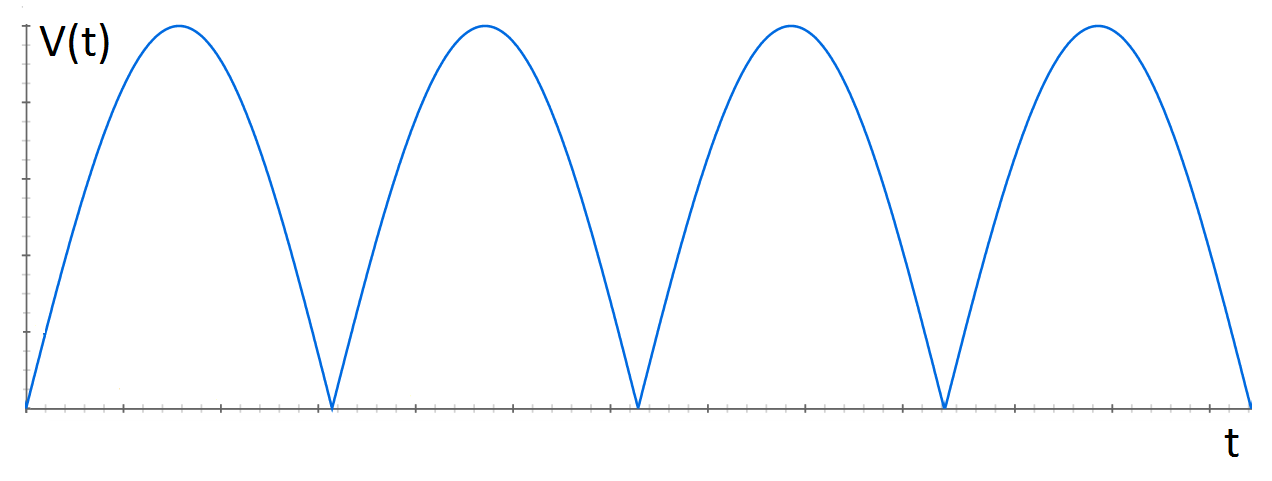
\includegraphics[width=\textwidth]{diagrams/rectifysin}
        \caption[Rectified A.C. output]{Output voltage after being sent through full wave rectifier.}
        \label{fig:rectified}
    \end{figure}
    
    In order to understand how this output is changing in Figure \ref{fig:data3}, only the maximum amplitudes will be analyzed. This means for each temperature, only the maximum value is considered. Experimentally, this can be done using a smoothing full wave rectifier. This could also be achieved by  programming the Arduino to only take the maximum value over some time period. 
    
    Data appear in straight vertical lines of the same temperature due to the different data collection rates for the thermocouple and voltage readings. This was done during the coding process because the thermocouple has a minimum response rate of 200ms, while data needed to be recorded for voltage over a shorter time period, such as 5ms. Random data points appear in the temperature range of less than about 140\degree C due to attempting to jump-start the engine, which was a necessary step. An increased number of data points appear around 350\degree C and greater because this is the temperature range that the engine sat at for the longest time period.